\documentclass[tikz,border=2pt]{standalone}

\usepackage{pgfplots}
\pgfplotsset{compat=1.18}

\begin{document}
	
	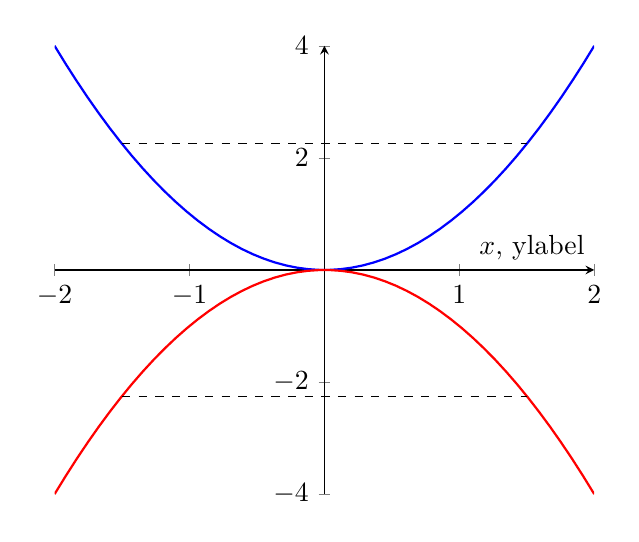
\begin{tikzpicture}
		\begin{axis}[
			axis lines = middle,
			xlabel = $x\text{,}$
			ylabel = {$y$},
			]
			% Convex function (f(x) = x^2)
			\addplot [thick,
			domain=-2:2,
			samples=50,
			color=blue,
			]
			{x^2};
			% Secant line on the convex function
			\draw [dashed] (-1.5,2.25) -- (1.5,2.25);
			% Concave function (g(x) = -x^2)
			\addplot [thick,
			domain=-2:2,
			samples=50,
			color=red,
			]
			{-x^2};
			% Secant line on the concave function
			\draw [dashed] (-1.5,-2.25) -- (1.5,-2.25);
		\end{axis}
	\end{tikzpicture}
	
\end{document}